\documentclass[conference]{IEEEtran}
\IEEEoverridecommandlockouts
\usepackage{cite}
\usepackage{amsmath,amssymb}
\usepackage{graphicx}
\usepackage{booktabs}
\usepackage{xcolor}
\usepackage{listings}
\usepackage{url}
\usepackage[hidelinks]{hyperref}
\lstset{basicstyle=\ttfamily\scriptsize,frame=single,columns=fullflexible,keepspaces=true}

\begin{document}

\title{Design and Verification of a Single-Cycle MIPS32 Processor with a Memory-Mapped Memory Interface in Verilog HDL\\
{\large Modern Computer Architecture -- Project Report (Phase I)}}

\author{
\IEEEauthorblockN{Keshav Rajput}
\IEEEauthorblockA{2401010222\\ Team Lead}
\and
\IEEEauthorblockN{Mayank Gupta}
\IEEEauthorblockA{2401010267}
\and
\IEEEauthorblockN{Gaurav Meena}
\IEEEauthorblockA{2401010169}
\and
\IEEEauthorblockN{Aaryan Gera}
\IEEEauthorblockA{2401010009}
\and
\IEEEauthorblockA{\textit{B.Tech CS\&AI, Newton School of Technology, Rishihood University, Sonipat, India}}
}

\maketitle

\begin{abstract}
This report presents the design, implementation and verification of a 32-bit single-cycle processor that executes a subset of the MIPS32 instruction set, together with a dedicated data-side memory interface. The core implements 27 instructions spanning R-type arithmetic, logical and shift operations, immediate arithmetic and logic, \texttt{lw}/\texttt{sw}, \texttt{beq}/\texttt{bne}, and \texttt{j}/\texttt{jal}/\texttt{jr}, which is sufficient to run recursive procedures that use the stack. The memory interface decodes every load/store address and routes it either to a 4~KB data RAM or to memory-mapped I/O registers (an output port, a cycle counter and a halt register). The design is written in synthesizable Verilog as 12 modules, verified with five self-checking unit testbenches and five assembly programs (a full instruction self-test, array sum, maximum search, recursive factorial and bubble sort) using a custom two-pass assembler. All tests pass, every instruction completes in one cycle (CPI~=~1), and a mutation experiment confirms that the self-test detects injected faults. Yosys synthesis for a Xilinx 7-series target maps the core to about 1{,}660 LUTs and 1{,}024 flip-flops.
\end{abstract}

\begin{IEEEkeywords}
MIPS, single-cycle processor, datapath, control unit, memory-mapped I/O, Verilog, RTL verification, computer architecture
\end{IEEEkeywords}

\section{Introduction}
A processor's datapath and control unit are where the instruction set architecture (ISA) meets hardware. Building one from scratch makes the link between an instruction's encoding and the signals that move data between registers, the ALU and memory concrete. The single-cycle organisation, in which each instruction is fetched, decoded, executed and written back within one clock period, is the standard starting point because every instruction's behaviour is visible in a single cycle of the waveform~\cite{patterson}.

The aim of this project is to implement a 32-bit single-cycle MIPS processor that executes arithmetic, memory and branch instructions, and to pair it with an explicit memory interface rather than wiring the data RAM directly into the datapath. The interface introduces address decoding and memory-mapped I/O (MMIO), which is how real processors reach peripherals. Phase~I delivers a working, verified and synthesised core; Phase~II will extend the analysis and results.

\section{Literature Review}
\textbf{The MIPS architecture.} MIPS grew out of the Stanford MIPS project of Hennessy \textit{et al.}~\cite{hennessy1982}, which argued that a simple, regular instruction set with fixed-length instructions and a load/store memory model lets the hardware be pipelined efficiently and moves complexity into the compiler. The commercial architecture is described by Kane and Heinrich~\cite{kane} and, for the 32-bit ISA used here, by the MIPS32 architecture manual~\cite{mips32}. Its three instruction formats (R, I and J), each 32 bits with the opcode in bits 31--26, make the decoder small, which is why MIPS remains the reference ISA for teaching processor design.

\textbf{Single-cycle and multi-cycle organisation.} Patterson and Hennessy~\cite{patterson} build the single-cycle datapath step by step, deriving a main decoder and a separate ALU-control decoder driven by a 2-bit ALUOp field. Harris and Harris~\cite{harris} give a synthesizable HDL realisation of the same design and point out its main limitation: the clock period must accommodate the slowest instruction (\texttt{lw}), which passes through instruction memory, register file, ALU, data memory and write-back. Multi-cycle and pipelined designs~\cite{patterson,hennessy_ca} remove this limitation but add state, pipeline registers and hazard handling. The single-cycle design is therefore the correct functional baseline against which later optimisations are measured.

\textbf{Memory interfaces and MMIO.} Textbook single-cycle cores usually connect an ideal data memory directly to the ALU output. Practical systems instead place a bus or address decoder between the core and its memories, and map peripherals into the address space so that ordinary loads and stores reach them~\cite{harris,hennessy_ca}. We adopt this approach, which keeps the core independent of the memory system and allows the same core to drive RAM, I/O or (in future) a cache.

\textbf{HDL and tools.} The design follows the IEEE~1364-2005 Verilog standard~\cite{verilog}. Simulation uses Icarus Verilog~\cite{icarus} and synthesis uses the open-source Yosys suite~\cite{yosys}, with resource estimates mapped to Xilinx 7-series primitives~\cite{ug474}.

\section{Proposed Solution}

\subsection{Supported Instruction Set}
Table~\ref{tab:isa} lists the 27 implemented instructions. The suggested set in the project brief (R-type, \texttt{lw}, \texttt{sw}, \texttt{beq}, \texttt{addi}, \texttt{j}) is extended with \texttt{bne}, shifts, logical immediates, \texttt{lui}, \texttt{slt(i/u)}, \texttt{jal} and \texttt{jr}. These additions allow realistic programs: \texttt{lui}/\texttt{ori} build 32-bit constants, and \texttt{jal}/\texttt{jr} with \texttt{lw}/\texttt{sw} on \texttt{\$sp} support recursive calls.

\begin{table}[htbp]
\caption{Implemented Instructions}
\label{tab:isa}
\centering
\footnotesize
\begin{tabular}{@{}ll@{}}
\toprule
Format & Instructions \\
\midrule
R (ALU) & add, addu, sub, subu, and, or, xor, nor, slt, sltu \\
R (shift) & sll, srl, sra \\
R (jump) & jr \\
I (ALU) & addi, addiu, andi, ori, xori, slti, lui \\
I (memory) & lw, sw \\
I (branch) & beq, bne \\
J & j, jal \\
\bottomrule
\end{tabular}
\end{table}

\subsection{Architecture Overview}
Fig.~\ref{fig:datapath} shows the processor. It uses a Harvard organisation: instructions come from a separate ROM and data accesses go through the memory interface, so fetch and data access can happen in the same cycle. On each rising clock edge the PC loads the next address. Within the cycle, the instruction is read, the register file supplies \texttt{rs} and \texttt{rt}, the immediate is extended, the ALU computes a result or address, the memory interface performs the access, and the write-back multiplexer selects the value written to the register file at the next edge.

\begin{figure*}[t]
\centering
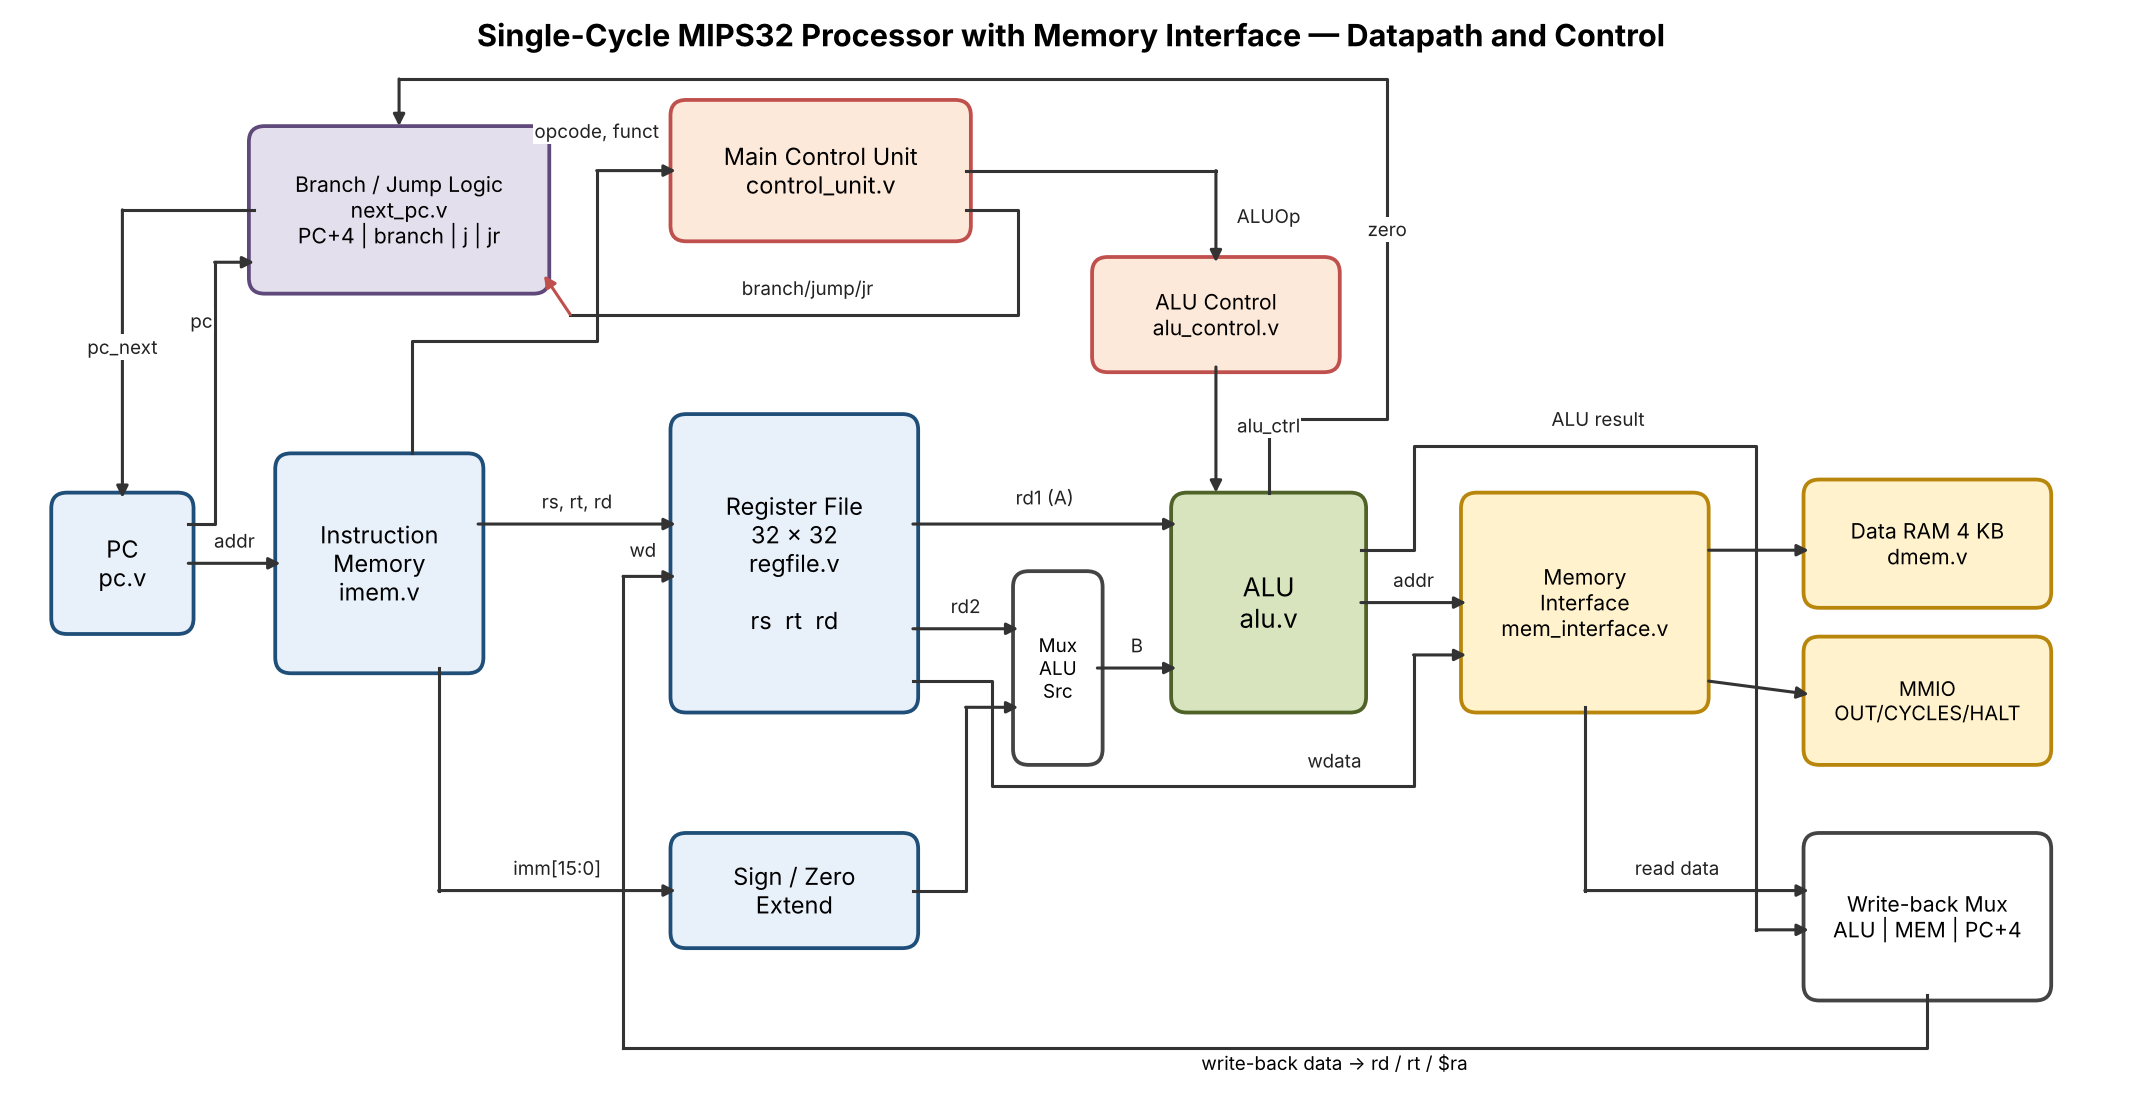
\includegraphics[width=0.92\textwidth]{datapath.png}
\caption{Datapath and control of the single-cycle MIPS32 processor with the memory interface. Red blocks are control, gold blocks form the memory subsystem.}
\label{fig:datapath}
\end{figure*}

\subsection{Module Description}
The RTL is divided into 12 modules (Table~\ref{tab:modules}). Each module has one job and is tested by its own testbench before integration.

\begin{table}[htbp]
\caption{RTL Modules}
\label{tab:modules}
\centering
\footnotesize
\begin{tabular}{@{}p{2.25cm}p{5.6cm}@{}}
\toprule
Module & Function \\
\midrule
\texttt{pc} & 32-bit PC register, synchronous reset, freezes on halt \\
\texttt{imem} & 1K-word instruction ROM loaded with \texttt{\$readmemh} \\
\texttt{control\_unit} & Main decoder: opcode/funct $\rightarrow$ 13 control signals \\
\texttt{alu\_control} & ALUOp + funct $\rightarrow$ 4-bit ALU operation \\
\texttt{regfile} & 32$\times$32 registers, 2 read / 1 write port, \texttt{\$0}=0 \\
\texttt{sign\_extend} & Sign- or zero-extension of the 16-bit immediate \\
\texttt{alu} & 12 operations, zero and overflow flags \\
\texttt{next\_pc} & PC+4, branch target, jump target, \texttt{jr} selection \\
\texttt{mem\_interface} & Address decoder, MMIO registers, misalignment check \\
\texttt{dmem} & 4~KB data RAM, synchronous write, combinational read \\
\texttt{mips\_cpu} & Core integration and write-back multiplexer \\
\texttt{mips\_top} & Core + instruction memory + memory interface \\
\bottomrule
\end{tabular}
\end{table}

\subsection{Control Unit}
Control is split into two levels, following~\cite{patterson}. The main decoder produces \textit{RegDst} (rt, rd or \$ra), \textit{ALUSrc}, \textit{MemToReg} (ALU, memory or PC+4), \textit{RegWrite}, \textit{MemRead}, \textit{MemWrite}, \textit{Branch}, \textit{BranchNE}, \textit{Jump}, \textit{JR}, \textit{ZeroExt} and a 3-bit \textit{ALUOp}. Because \texttt{jr} is an R-type instruction, the decoder also looks at the funct field. A 3-bit ALUOp (instead of the 2-bit field in the textbook) lets I-type logical instructions and \texttt{lui} select their ALU operation without a funct field. Unknown opcodes set an \textit{illegal} flag and are executed as NOPs.

\subsection{Branch and Jump Logic}
The next PC is selected with the priority \texttt{jr} $>$ \texttt{j/jal} $>$ taken branch $>$ PC+4. A branch is taken when $(Branch \land Z) \lor (BranchNE \land \lnot Z)$, where $Z$ is the ALU zero flag after computing $rs - rt$. The branch target is $PC{+}4 + (\mathrm{sext}(imm) \ll 2)$ and the jump target is $\{PC{+}4[31{:}28], index, 00\}$. For \texttt{jal} the write-back mux writes PC+4 to \$31.

\subsection{Memory Interface}
The memory interface sits between the core's data bus and the memory system. It decodes the ALU-computed address as follows:
\begin{itemize}
\item \texttt{0x0000\_0000--0x0000\_0FFF}: data RAM (1024 words);
\item \texttt{0x0000\_FFF0}: \textit{IO\_OUT}, a write latches a value on the output port and pulses \textit{io\_out\_valid};
\item \texttt{0x0000\_FFF8}: \textit{IO\_CYCLES}, a read returns the cycle count since reset;
\item \texttt{0x0000\_FFFC}: \textit{IO\_HALT}, a write stops the processor.
\end{itemize}
Writes to the I/O region never reach the RAM, and accesses whose address is not word-aligned raise a \textit{misaligned} flag. The RAM writes on the clock edge and reads combinationally, which a single-cycle design needs so that \texttt{lw} can complete in the same cycle. The \texttt{\$sp} register is reset to \texttt{0x0FFC}, the top of RAM, so the stack grows down from the end of data memory.

\subsection{Toolflow}
A two-pass Python assembler (\texttt{scripts/mips\_asm.py}) turns assembly into hex images for \texttt{\$readmemh}. It supports labels, \texttt{.text}/\texttt{.data}/\texttt{.word}/\texttt{.space}, and the pseudo-instructions \texttt{li}, \texttt{la}, \texttt{move}, \texttt{nop}, \texttt{b}, \texttt{print} and \texttt{halt}; the last two expand to stores to the MMIO registers. A regression script (\texttt{scripts/run\_tests.py}, run by \texttt{make test}) assembles every program, simulates it with Icarus Verilog, compares the values written to \textit{IO\_OUT} against expected results and runs all unit testbenches.

\section{Preliminary Results}

\subsection{Verification}
Table~\ref{tab:results} summarises the regression results. The program \texttt{full\_test.s} checks each instruction class and branches to a failure handler that prints \texttt{0xBAD0\_00NN} (NN = failing test number) on any mismatch; on success it prints \texttt{0x600D}. The factorial program exercises recursion through \texttt{jal}/\texttt{jr} with a software shift-and-add multiplier, and bubble sort exercises dense load/store traffic with signed comparisons.

\begin{table}[htbp]
\caption{Regression Results (Icarus Verilog)}
\label{tab:results}
\centering
\footnotesize
\begin{tabular}{@{}lll@{}}
\toprule
Test & Output on IO\_OUT & Cycles \\
\midrule
\texttt{full\_test} & \texttt{0x600D} (pass) & 97 \\
\texttt{array\_sum} & 55 & 85 \\
\texttt{max\_search} & 97 & 73 \\
\texttt{factorial} & 1, 2, 6, 24, 120, 720, 5040 & 922 \\
\texttt{bubble\_sort} & $-7$, 0, 3, 9, 15, 22, 41, 88 & 364 \\
\midrule
Unit tests & ALU (15), RegFile (66), Control (14), & all pass \\
 & Next-PC (7), Memory interface & \\
\bottomrule
\end{tabular}
\end{table}

Because the design is single-cycle, the number of cycles equals the number of instructions executed in every program (CPI~=~1). To check that the self-test can actually detect faults, we injected a bug that made \texttt{sra} behave as a logical shift. The program then printed \texttt{0xBAD0\_0005}, pointing to the shift test.

Fig.~\ref{fig:wave} shows the first 26 cycles of \texttt{array\_sum}. Cycles 0--5 set up the array pointer and length (with \textit{MemRead} high for \texttt{lw} in cycle 3), and from cycle 6 the loop body repeats every seven cycles; the jump at PC \texttt{0x34} returns to the loop test at \texttt{0x1C}.

\begin{figure}[htbp]
\centering
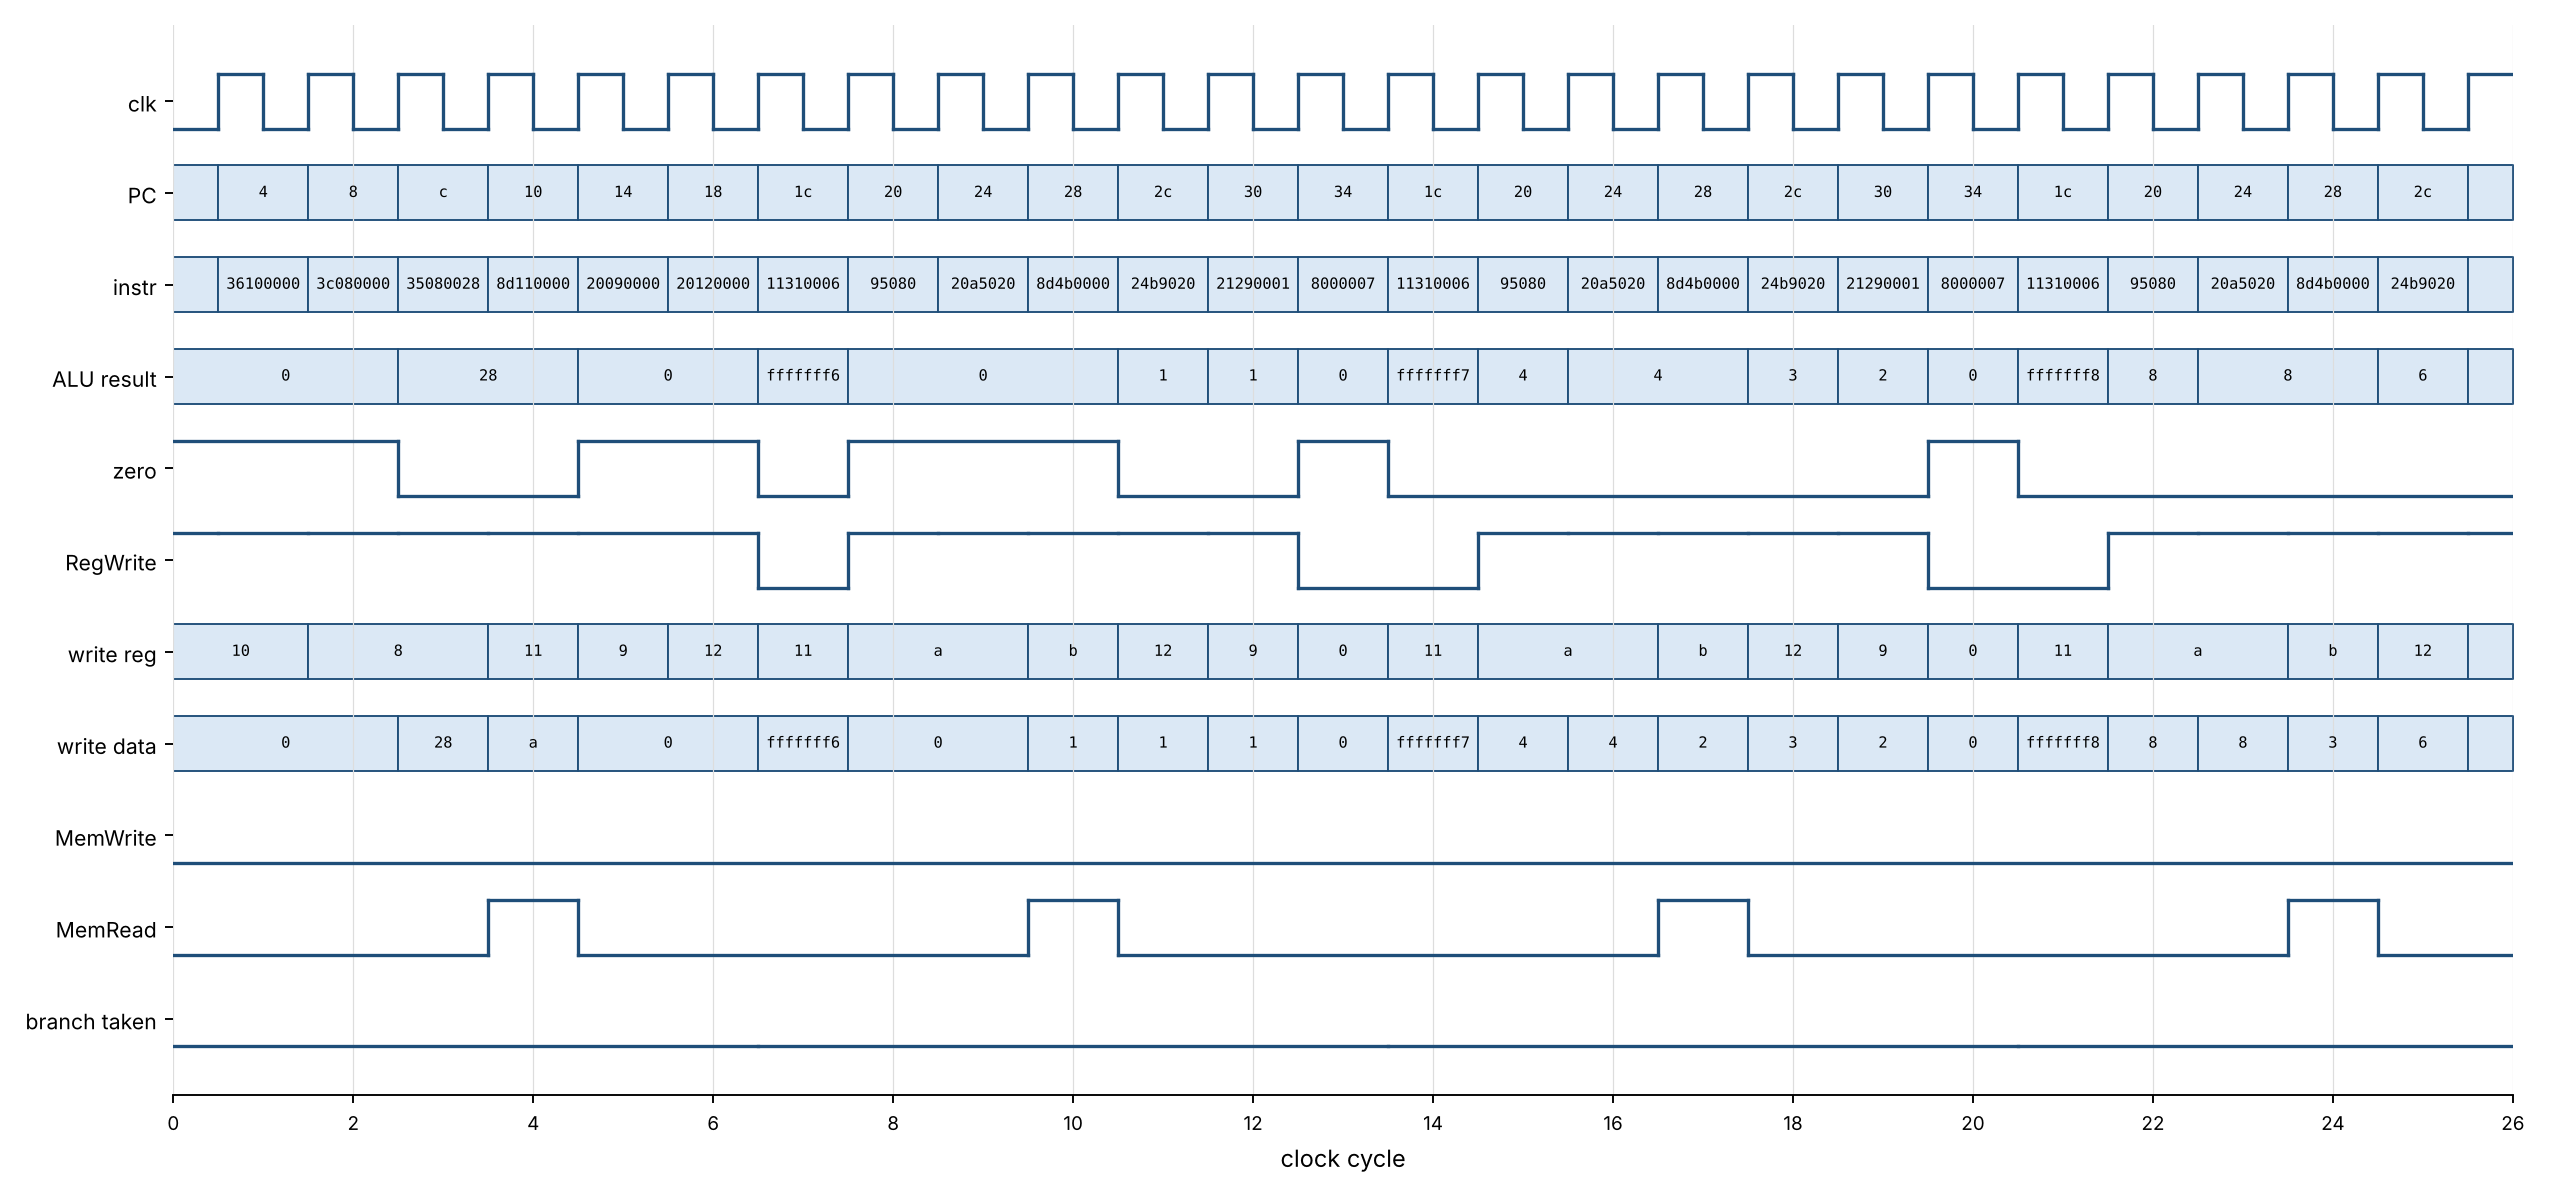
\includegraphics[width=\columnwidth]{wave_array_sum.png}
\caption{Simulation waveform for \texttt{array\_sum}: PC, instruction, ALU result and control signals per cycle.}
\label{fig:wave}
\end{figure}

\subsection{Synthesis}
The core (datapath and control, excluding the memory arrays, which map to block RAM) was synthesised with Yosys for a Xilinx 7-series target. It uses about 1{,}660 LUTs, 1{,}024 flip-flops, 375 wide multiplexers (MUXF7/F8) and 38 CARRY4 chains. The flip-flops are the 32$\times$32 register file; because it has a synchronous reset, it is not inferred as distributed RAM. The critical path is the \texttt{lw} path: instruction memory $\rightarrow$ register file $\rightarrow$ ALU adder $\rightarrow$ data memory $\rightarrow$ write-back mux $\rightarrow$ register file setup.

\section{Individual Contributions}
\begin{itemize}
\item \textbf{Keshav Rajput (Team Lead):} overall architecture and memory map; main control unit and ALU-control decoder; core integration (\texttt{mips\_cpu}, \texttt{mips\_top}) and write-back logic; system and control-unit testbenches; Yosys synthesis; repository setup; report.
\item \textbf{Mayank Gupta:} ALU with flags, 32$\times$32 register file and sign/zero-extension unit, with their unit testbenches (ALU and register file).
\item \textbf{Gaurav Meena:} program counter, instruction memory, data memory and the memory interface (address decoder, MMIO registers and misalignment detection), with the memory-interface testbench.
\item \textbf{Aaryan Gera:} branch/jump next-PC logic and its testbench; MIPS assembler; the five test programs; regression runner and waveform plotting scripts.
\end{itemize}

\section{Conclusion and Phase II Plan}
A complete single-cycle MIPS32 processor with a memory-mapped memory interface has been implemented and verified, and it runs recursive and memory-intensive programs correctly. Phase~II will add static timing estimates and maximum clock frequency on an FPGA target, a performance comparison of the benchmark programs, byte and halfword loads/stores (\texttt{lb}, \texttt{lbu}, \texttt{sb}) with byte enables in the memory interface, and a final report with full results and discussion.

\begin{thebibliography}{00}
\bibitem{patterson} D. A. Patterson and J. L. Hennessy, \textit{Computer Organization and Design: The Hardware/Software Interface}, 5th ed. Waltham, MA, USA: Morgan Kaufmann, 2014.
\bibitem{harris} D. M. Harris and S. L. Harris, \textit{Digital Design and Computer Architecture}, 2nd ed. Waltham, MA, USA: Morgan Kaufmann, 2013.
\bibitem{hennessy_ca} J. L. Hennessy and D. A. Patterson, \textit{Computer Architecture: A Quantitative Approach}, 6th ed. Cambridge, MA, USA: Morgan Kaufmann, 2019.
\bibitem{hennessy1982} J. Hennessy, N. Jouppi, F. Baskett, T. Gross, and J. Gill, ``Hardware/software tradeoffs for increased performance,'' in \textit{Proc. Symp. Architectural Support for Programming Languages and Operating Systems (ASPLOS)}, 1982, pp. 2--11.
\bibitem{kane} G. Kane and J. Heinrich, \textit{MIPS RISC Architecture}. Englewood Cliffs, NJ, USA: Prentice Hall, 1992.
\bibitem{mips32} MIPS Technologies, \textit{MIPS32 Architecture for Programmers, Volume II: The MIPS32 Instruction Set}, Rev. 6.06, 2016.
\bibitem{verilog} \textit{IEEE Standard for Verilog Hardware Description Language}, IEEE Std 1364-2005, 2006.
\bibitem{icarus} S. Williams, ``Icarus Verilog,'' [Online]. Available: \url{https://steveicarus.github.io/iverilog/}
\bibitem{yosys} C. Wolf, ``Yosys Open SYnthesis Suite,'' [Online]. Available: \url{https://yosyshq.net/yosys/}
\bibitem{ug474} Xilinx Inc., \textit{7 Series FPGAs Configurable Logic Block User Guide}, UG474, v1.8, 2016.
\end{thebibliography}

\end{document}
